% --- (1) Einseitiges Dokument ---
\documentclass[a4paper,12pt]{scrreprt}
\usepackage{listings}
\usepackage{amsmath}
% Grafiken im Fließtext
\usepackage{floatflt}
\usepackage[pdftex]{graphicx}
% tikz => Diagramme
\usepackage{tikz}
% Grafiken mit Hilfe von [H] an der definierten Stelle platzieren
\usepackage{here}
% UML-Diagramme mit Hilfe von tikz
\usepackage[
% school,
% simplified
]{pgf-umlcd}
\RequirePackage[utf8]{inputenc}
% CKL: Dieses LaTeX-Dokument ist für einen einseitgen Druck ausgelegt.
% CKL: Dafür sorgen, dass die Fußnotennummerierung nicht mit jedem Kapitel neu beginnt
\usepackage{remreset}
\makeatletter
\@removefromreset{footnote}{chapter}
\makeatother

% ==========[ Einstellungen laden ]==========

\input{wissenschaftlich_arbeiten_latex.settings}


\begin{document}


% ==========[ Deckblatt mit Angaben zum Dokument ]==========

\titelSeiteDaten
{Bachelor-Thesis} % Art der Arbeit
{}
{Ostfalia Hochschule für angewandte Wissenschaften} % Name der Hochschule
{Informatik} % Fachbereichsname
{IT-Management} % Name des Studiengangs
{Entwicklung einer domönspezifischen Sprache zur Unterstützung der Angebotserstellung} % Titel der Arbeit
{}
{}
\titelSeiteNamen
{Stephan Elvers} % Name des Autors
{70382189} % Matrikel-Nummer
{Prof. Dr. Ina Schiering} % Name des Erstprüfers
{B.Sc Christopher Klein}
{0. Mai 2019} % Abgabedatum

% ==========[ Schriftgroesse und Zeilenhoehe ]==========

\fontsize{12pt}{13pt}\selectfont


% ==========[ Inhaltsverzeichnis ]==========

% Gliederungstiefe des Inhaltsverzeichnisses
\setcounter{tocdepth}{1}

% Inhaltsverzeichnis
\tableofcontents

% ==========[ Beginn des eigentlichen Inhaltes ]==========

% Layout pruefen und Nummerierung anpassen
\leerSeiteInhalt


% Blocksatz aktivieren
\sloppy

\chapter{Abstrakt}
\index{Abstrakt}
In Softwareprojekten wird der Großteil des Quellcodes von Hand geschrieben, obwohl sich viele der notwendigen Artefakte aus vorhandenen Informationen automatisiert generieren ließen. Die Generierung von Quellcode reduziert die Fehleranfälligkeit innerhalb der zu entwicklenden Anwendung und sorgt dafür, dass mehr Zeit in die Implementierung der Geschäftslogik investiert werden kann.
\\
\\
In dieser Bachelorarbeit wird untersucht.....
\chapter{Einleitung}
\index{Einleitung}
"Write Code That Writes Codes" \cite{ht2006}
 \textit{Kursiv}

\section{Aufgabenstellung}
unterkapitel
\\
\\
Das im Rahmen dieser Bachelorarbeit entstehende Eclipse Plug-in soll dabei so entwickelt werden, dass neue Generatoren für Code-Fragmente einfach integriert werden können.
\section{Motivation}
Auslöser für diese Bachelor-Arbeit ist ein abgeschlossenes Software-Projekt gewesen, in dem bereits Xtext im kleinen Rahmen verwendet wurde.
Die dabei erstellte domänenspezifische Sprache (\textit{Domain Specific Language}, \textit{DSL}) beschrieb die Domänen-Objekte mit ihren Attributen, die mit Hilfe von Xtext in C\#-Quellcode umgewandelt wurden.
Die DSL wurde zwar nur für grundlegende Transformationen benutzt, dennoch lag der dadurch entstandene Mehrwert auf der Hand. Es entstand eine einheitliche Basis für Dokumentation und Quellcode. Die Zeit, die für alltägliche Programmierarbeiten wie dem Implementieren von Entitäten oder der Datenzugriffsschicht anfiel, wurde auf ein Minimum verringert.
\section{Vorgehen}
 Kapitel \ref{ch:technologien}  <- Verweis auf anderes Kapitel
\\
\\
Liste
\begin{itemize}
	\item Pfadangaben und Dateinamen werden in kursiver Schrift dargestellt, z.B. \textit{src/plugin.xml}
	\item Quellcode wird in Verbatim dargestellt, z.B. \texttt{addComponent(...)}   <--   Fett/Verbatim
	\item ....
\end{itemize}

\chapter{Ausgangssituation}
\section{Kontext}

\section{Aktueller Entwicklungsprozess}
Im Folgenden soll ein Einblick in den aktuell vorhandenen Softwareent\-wick\-lungs\-prozess bei der NeosIT GmbH gegeben werden. Eine detaillierte Beschreibung würde den Rahmen dieser Arbeit sprengen.

\subsection{Requirements Engineering}
 unterunterkapitel



\footnote{DAL bzw. DAO-Entwurfsmuster}rt. 
Tabelle \ref{frameworks} 


\begin{table}[h]
\begin{tabular}{l|l|l}
Komponente 	& 		C\# 		&	 Java\\
\hline
Logging 	& NLog oder log4net & log4j \\
Dependency Injection & Unity oder Spring.NET & Spring oder Guice \\
MVC & ASP.NET MVC 2/3 & Spring MVC \\
Scheduling 	& Quartz.NET 		& Quartz 	\\
Messaging Queue & ActiveMQ 		& ActiveMQ 	 \\
AOP & Unity & AspectJ \\
Testing & Xunit & JUnit \\
\end{tabular}
\caption{\label{frameworks}Eingesetzte Frameworks}
\end{table}


\subsection{Generierung eines Mockups}
\label{sub:gen_prototyp}

\begin{verbatim}
ALTER TABLE xyz ADD COLUMN nachname char(255);
\end{verbatim}




\begin{figure}[h]
	\centering
		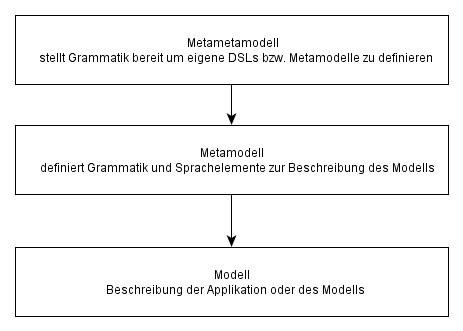
\includegraphics[width=300px]{diagramme/meta-meta-modell.png}
		\caption{Modell,  Metamodell und Metametamodell}
		\label{fig:meta-meta-modell}
\end{figure}


\textbf{ohne} <--- Fett

...... \verb+Module+ implementiere ...   ODER .....Variablen \verb-artefakt- gespeichert werden.... <----  Verbatism im fließtext




\subsection{Erstellung einer neuen DSL}
\newcommand{\paketname}[0]{{\textit{\${paket.name}}}}
\newcommand{\dslname}[0]{{\textit{\${dsl-name}}}}
\begin{itemize}
	\item Der Benutzer erstellt innerhalb der Eclipse-Umgebung ein neues Xtext-DSL-Projekt.
	Dabei muss er den Namen der DSL \dslname, sowie den Paketnamen der DSL \paketname\ definieren.
	\item Das Eclipse Plug-in des Xtext-Frameworks generiert daraufhin automatisch drei Eclipse Plug-ins:
	\begin{itemize}
		\item \paketname: Grundgerüst für das DSL-Backend. Dieses enthält den Parser, Lexer, Formatter,  Metamodell, Scoping- und Validation-Provider. Der generierte Quellcode ist standardmäßig nicht abhängig von der Eclipse-Laufzeitumgebung und kann auch in Konsolen- oder Webanwendungen wiederverwendet werden.
		\item \paketname.test: Grundgerüst für das Ausführen von Unittests
		\item \paketname.ui: Grundgerüst für das User Interface. Dies beinhaltet unter anderem Content Assistents, Quickfixing und Outline Views. Der generierte Quellcode hängt dabei 

\end{itemize}
\end{itemize}

\emph{src-gen} erzeugt. 
\\
\\

% ==========[ An dieser Stelle beginnt der Anhang ]==========

% Anhang
\appendix

% Layout pruefen und Nummerierung anpassen
\leerSeiteAnhang

\chapter*{Eidesstattliche Erklärung}
Hiermit versichere ich, dass ich die vorliegende Arbeit selbständig verfasst und keine anderen als die angegebenen Quellen und Hilfsmittel benutzt habe. Ich versichere, dass ich alle wörtlich oder sinngemäß aus anderen Werken übernommenen Aussagen als solche gekennzeichnet habe, und dass die eingereichte Arbeit weder vollständig noch in wesentlichen Teilen Gegenstand eines anderen Prüfungsverfahrens gewesen ist.




\vspace*{3em}

\newcommand*{\SignatureAndDate}[1]{
	\par\noindent\makebox[52mm]{\hrulefill}     \hfill\makebox[65mm]{\hrulefill}
	\par\noindent\makebox[52mm][l]{Ort, Datum}	\hfill\makebox[62mm][l]{#1}
}

\SignatureAndDate{Unterschrift}
	
% ==========[ Abkuerzungsverzeichnis ]==========

\begin{abkuerzung}\label{abk}

% Bitte achten Sie auf die alphabetische Sortierung!
\abkuerzungEintrag{API}{Application Programming Interface}
\abkuerzungEintrag{CRUD}{Create, Read, Update, Delete}
\abkuerzungEintrag{CSS}{Cascading Stylesheet}
\abkuerzungEintrag{CSV}{Comma-separated values}
\abkuerzungEintrag{DAL}{Data Access Layer}
\abkuerzungEintrag{DAO}{Data Access Object}
\abkuerzungEintrag{DBMS}{Datenbank Management System}
\abkuerzungEintrag{DDL}{Data Definition Language}
\abkuerzungEintrag{DET}{Data Element Type}
\abkuerzungEintrag{DSL}{Domain Specific Language}
\abkuerzungEintrag{ELF}{External Logical File}
\abkuerzungEintrag{EMF}{Eclipse Modeling Framework}
\abkuerzungEintrag{FTR}{File Type Reference}
\abkuerzungEintrag{FPA}{Function Point-Analyse}
\abkuerzungEintrag{HTML}{Hypertext Markup Language}
\abkuerzungEintrag{IDE}{Integrated Development Environment}
\abkuerzungEintrag{ILF}{Internal Logical File}
\abkuerzungEintrag{JDT}{Java Development Toolkit}
\abkuerzungEintrag{JPA}{Java Persistence API}
\abkuerzungEintrag{JVM}{Java Virtual Machine}
\abkuerzungEintrag{MDA}{Model Driven Architecture}
\abkuerzungEintrag{MWE}{Model Workflow Engine}
\abkuerzungEintrag{PDE}{Plug-in Development Environment}
\abkuerzungEintrag{PDT}{PHP Development Toolkit}
\abkuerzungEintrag{POJO}{Plain Old Java Object}
\abkuerzungEintrag{RET}{Record Element Type}
\abkuerzungEintrag{SCM}{Source Code Management}
\abkuerzungEintrag{SWT}{Standard Widget Toolkit}
\abkuerzungEintrag{TDD}{Test Driven Development}
\abkuerzungEintrag{UML}{Unified Modeling Language}


\end{abkuerzung}



% ==========[ Verzeichnisse ]==========

% Nicht gewuenschte Verzeichnisse koennen auskommentiert werden
% Abbildungsverzeichnis und Tabellenverzeichnis auf einer Seite, da zu wenig Grafiken bzw. Tabellen vorhanden
\listoffigures
\addcontentsline{toc}{chapter}{Abbildungs- und Tabellenverzeichnis}
\begingroup
\let\clearpage\relax
\listoftables
\endgroup



% ==========[ Glossar ]==========

\begin{glossar}\label{glossar}

% Bitte achten Sie auf die alphabetische Sortierung!
\glossarEintrag{Annotation}{Annotationen dienen dazu, Metadaten innerhalb einer Programmiersprache oder DSL zu hinterlegen.}
\glossarEintrag{Artefakt}{Ein Artefakt stellt im Rahmen dieser Arbeit ein oder mehre Quellcodedateien dar, die automatisiert erzeugt worden sind.}
\glossarEintrag{Artefakt-Generator}{Ein Plug-in zur automatisierten Erstellung von Artefakten bzw. Quellcode. Der Generator nutzt dabei das Modell der DSL als Basis.}
\glossarEintrag{Domäne}{Als Domäne wird der Bereich bezeichnet, in dem eine domänenspezifische Sprache eingesetzt wird.}
\glossarEintrag{Eclipse}{Eine Entwicklungsumgebung für Java und andere Programmiersprachen}
\glossarEintrag{Function Point-Analyse}{Methodik, die zur Aufwandsabschätzung von Softwareprojekten angewandt werden kann.}
\glossarEintrag{Lambda-Ausdruck}{Ein Lambda-Ausdruck stellt eine anonyme Funktion dar, die an eine Methode übergeben werden kann.}
\glossarEintrag{Mockup}{Beispielhafte Darstellung einer Anwendung ohne oder mit wenig Funktionalität.}
\glossarEintrag{Modell}{Das Modell bildet mit Hilfe der DSL die Anforderungen einer Domäne in einer textuellen Form ab.}
\glossarEintrag{transient}{Ein Element (Domäne, Attribut o.ä.), das zur Laufzeit nicht in einer Datenbank persistiert wird.}
\end{glossar}



% ==========[ Literaturverzeichnis ]==========

\nocite{*}
\addcontentsline{toc}{chapter}{Literaturverzeichnis}
\bibliography{wissenschaftlich_arbeiten_latex}



% ==========[ Index ]==========

% Bitte beachten Sie zur Erstellung des Index die Hinweise in der
% beiligenden Anleitung im PDF-Format, da sonst kein Index fuer
% das Dokument erstellt und ausgegeben wird.

% \indexInhalt
% \printindex

\end{document}

